\documentclass[12pt, a4paper,  BCOR=8.25mm, DIV=15]{scrartcl}\usepackage[]{graphicx}\usepackage[]{color}
%% maxwidth is the original width if it is less than linewidth
%% otherwise use linewidth (to make sure the graphics do not exceed the margin)
\makeatletter
\def\maxwidth{ %
  \ifdim\Gin@nat@width>\linewidth
    \linewidth
  \else
    \Gin@nat@width
  \fi
}
\makeatother

\definecolor{fgcolor}{rgb}{0.345, 0.345, 0.345}
\newcommand{\hlnum}[1]{\textcolor[rgb]{0.686,0.059,0.569}{#1}}%
\newcommand{\hlstr}[1]{\textcolor[rgb]{0.192,0.494,0.8}{#1}}%
\newcommand{\hlcom}[1]{\textcolor[rgb]{0.678,0.584,0.686}{\textit{#1}}}%
\newcommand{\hlopt}[1]{\textcolor[rgb]{0,0,0}{#1}}%
\newcommand{\hlstd}[1]{\textcolor[rgb]{0.345,0.345,0.345}{#1}}%
\newcommand{\hlkwa}[1]{\textcolor[rgb]{0.161,0.373,0.58}{\textbf{#1}}}%
\newcommand{\hlkwb}[1]{\textcolor[rgb]{0.69,0.353,0.396}{#1}}%
\newcommand{\hlkwc}[1]{\textcolor[rgb]{0.333,0.667,0.333}{#1}}%
\newcommand{\hlkwd}[1]{\textcolor[rgb]{0.737,0.353,0.396}{\textbf{#1}}}%
\let\hlipl\hlkwb

\usepackage{framed}
\makeatletter
\newenvironment{kframe}{%
 \def\at@end@of@kframe{}%
 \ifinner\ifhmode%
  \def\at@end@of@kframe{\end{minipage}}%
  \begin{minipage}{\columnwidth}%
 \fi\fi%
 \def\FrameCommand##1{\hskip\@totalleftmargin \hskip-\fboxsep
 \colorbox{shadecolor}{##1}\hskip-\fboxsep
     % There is no \\@totalrightmargin, so:
     \hskip-\linewidth \hskip-\@totalleftmargin \hskip\columnwidth}%
 \MakeFramed {\advance\hsize-\width
   \@totalleftmargin\z@ \linewidth\hsize
   \@setminipage}}%
 {\par\unskip\endMakeFramed%
 \at@end@of@kframe}
\makeatother

\definecolor{shadecolor}{rgb}{.97, .97, .97}
\definecolor{messagecolor}{rgb}{0, 0, 0}
\definecolor{warningcolor}{rgb}{1, 0, 1}
\definecolor{errorcolor}{rgb}{1, 0, 0}
\newenvironment{knitrout}{}{} % an empty environment to be redefined in TeX

\usepackage{alltt}
\usepackage[utf8]{inputenc}

\newenvironment{itemizz}%
  {\begin{itemize}%
    \setlength{\itemsep}{2pt}%
    \setlength{\parskip}{2pt}}%
  {\end{itemize}}

\newcommand{\txtt}[1]{{\texttt{#1}}}
\IfFileExists{upquote.sty}{\usepackage{upquote}}{}
\begin{document}
%\VignetteEngine{knitr::knitr}
%\VignetteIndexEntry{Data (Set 4)}



\title{4: Data}
\author{John H Maindonald}
\maketitle

\vspace*{-24pt}

\begin{knitrout}
\definecolor{shadecolor}{rgb}{0.969, 0.969, 0.969}\color{fgcolor}\begin{kframe}
\begin{alltt}
\hlstd{fig4.1} \hlkwb{<-} \hlkwa{function}\hlstd{()\{}
\hlcom{## ---- date-labs ----}
\hlcom{## Labeling of graph: data frame jobs (DAAG)}
\hlkwd{library}\hlstd{(DAAG,} \hlkwc{quietly}\hlstd{=}\hlnum{TRUE}\hlstd{);} \hlkwd{library}\hlstd{(lattice)}
\hlstd{fromdate} \hlkwb{<-} \hlkwd{as.Date}\hlstd{(}\hlstr{"1Jan1995"}\hlstd{,} \hlkwc{format}\hlstd{=}\hlstr{"%d%b%Y"}\hlstd{)}
\hlstd{startofmonth} \hlkwb{<-} \hlkwd{seq}\hlstd{(}\hlkwc{from}\hlstd{=fromdate,} \hlkwc{by}\hlstd{=}\hlstr{"1 month"}\hlstd{,} \hlkwc{length}\hlstd{=}\hlnum{24}\hlstd{)}
\hlstd{atdates} \hlkwb{<-} \hlkwd{seq}\hlstd{(}\hlkwc{from}\hlstd{=fromdate,} \hlkwc{by}\hlstd{=}\hlstr{"6 month"}\hlstd{,} \hlkwc{length}\hlstd{=}\hlnum{4}\hlstd{)}
\hlkwd{xyplot}\hlstd{(BC} \hlopt{~} \hlstd{startofmonth,} \hlkwc{data}\hlstd{=jobs,}
       \hlkwc{scale}\hlstd{=}\hlkwd{list}\hlstd{(}\hlkwc{x}\hlstd{=}\hlkwd{list}\hlstd{(}\hlkwc{at}\hlstd{=atdates,}
                         \hlkwc{labels}\hlstd{=}\hlkwd{format}\hlstd{(atdates,} \hlstr{"%b%y"}\hlstd{))))}
\hlstd{\}}
\end{alltt}
\end{kframe}
\end{knitrout}
\vspace*{-24pt}

\begin{figure}
\begin{knitrout}
\definecolor{shadecolor}{rgb}{0.969, 0.969, 0.969}\color{fgcolor}\begin{kframe}
\begin{alltt}
\hlkwd{fig4.1}\hlstd{()}
\end{alltt}
\end{kframe}

{\centering 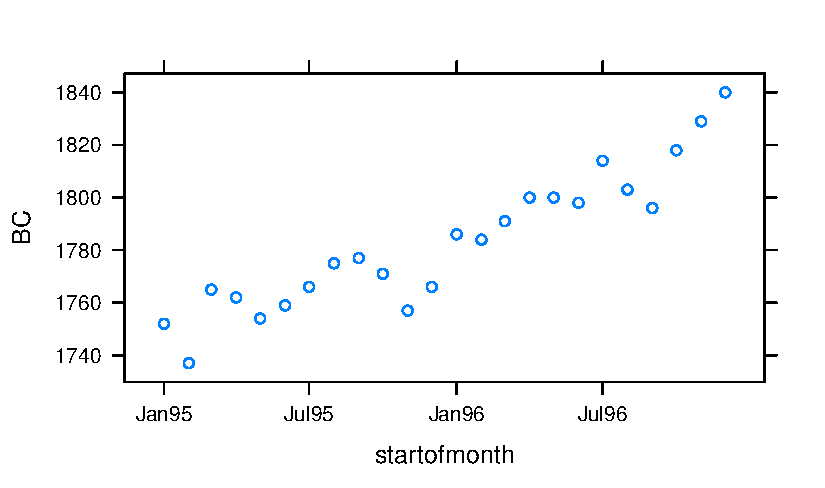
\includegraphics[width=0.65\textwidth]{figs/data-fig4_1e-1} 

}



\end{knitrout}
\caption{Dates are used to label the $x$-axis}\label{fig:simplatparam}
\end{figure}

\end{document}
